\documentclass[xetex]{beamer}
\usepackage{fontspec}
\usepackage{mathtools}
\usepackage{unicode-math}
\usepackage{tikz}
\usetikzlibrary{trees}
\usepackage{mathpartir}
\usepackage{parskip}
\usepackage{minted}
\usepackage{csquotes}
\usepackage{tcolorbox}
\usepackage{biblatex} % TODO style w/o quotation marks

\setmainfont{XITS}
\setmathfont{XITS Math}
\setsansfont[Scale=MatchLowercase]{DejaVu Sans}
\setmonofont[Scale=MatchLowercase]{DejaVu Sans Mono}

\addbibresource{lit.bib}

% Emoji images are from
% https://github.com/joypixels/emoji-assets/blob/master/png/128
\newlength{\emojiheight}
\settoheight{\emojiheight}{H}
\newcommand{\good}{
\includegraphics[height=\emojiheight]{images/1f973}}
\newcommand{\bad}{
\includegraphics[height=\emojiheight]{images/1fae4}}

\setbeamertemplate{navigation symbols}{}
\setbeamertemplate{itemize item}{\Large\textbullet}
\setbeamertemplate{itemize subitem}{\Large\textbullet}
\setbeamertemplate{itemize subsubitem}{\Large\textbullet}

\tcbset{frame empty}

\setminted[lean4]{extrakeywords={aesop cases add aesop? intro simp simp_all only split apply}}
\newmintinline[lean]{lean4}{bgcolor={},ignorelexererrors=true}
\newminted[leancode]{lean4}{bgcolor={},ignorelexererrors=true,fontsize=\footnotesize,autogobble}
\BeforeBeginEnvironment{leancode}{\begin{tcolorbox}}
\AfterEndEnvironment{leancode}{\end{tcolorbox}}
\usemintedstyle{xcode}

\setlength{\parskip}{1em}
\setlength{\tabcolsep}{0.5em}

% Source: https://tex.stackexchange.com/questions/55806/mindmap-tikzpicture-in-beamer-reveal-step-by-step/55849#55849
%
% Keys to support piece-wise uncovering of elements in TikZ pictures:
% \node[visible on=<2->](foo){Foo}
% \node[visible on=<{2,4}>](bar){Bar}   % put braces around comma expressions
%
% Internally works by setting opacity=0 when invisible, which has the
% advantage (compared to \node<2->(foo){Foo} that the node is always there, hence
% always consumes space plus that coordinate (foo) is always available.
%
% The actual command that implements the invisibility can be overridden
% by altering the style invisible. For instance \tikzsset{invisible/.style={opacity=0.2}}
% would dim the "invisible" parts. Alternatively, the color might be set to white, if the
% output driver does not support transparencies (e.g., PS)
\tikzset{
  invisible/.style={opacity=0},
  visible on/.style={alt={#1{}{invisible}}},
  alt/.code args={<#1>#2#3}{%
    \alt<#1>{\pgfkeysalso{#2}}{\pgfkeysalso{#3}} % \pgfkeysalso doesn't change the path
  },
}

\renewcommand{\iff}{\leftrightarrow}
\newcommand{\com}{,\,}
\newcommand{\orange}[1]{\textcolor{orange}{#1}}
\newcommand{\blue}[1]{{\usebeamercolor[fg]{palette primary} #1}}
\newcommand{\grey}[1]{\textcolor{lightgrey}{#1}}
\newcommand{\mv}[1]{\ensuremath{\mathit{?#1}}}
\newcommand{\rulename}[1]{\textrm{#1}}
\newcommand{\rulelabel}[1]{\quad \text{\rulename{#1}}}
\newcommand{\Expr}{\ensuremath{\mathbb{E}}}
\newcommand{\Hyps}{\ensuremath{\mathbb{H}}}
\newcommand{\Matches}{\ensuremath{\mathbb{M}}}
\newcommand{\Slots}{\ensuremath{\mathbb{S}}}
\newcommand{\Vars}{\ensuremath{\mathbb{V}}}
\newcommand{\Pow}[1]{\ensuremath{\mathcal{P}(#1)}}
\newenvironment{rapppic}{\begin{tikzpicture}[outer sep=auto, level distance=3em]}{\end{tikzpicture}}
\newenvironment{rapp}{%
  \begin{tcolorbox}
  \begin{center}
  \begin{rapppic}
}{
  \end{rapppic}
  \end{center}
  \end{tcolorbox}%
}

\begin{document}

\title{Aesop: White-Box Automation for Lean~4}
\author{Jannis Limperg\\ University of Munich (LMU)\\ \href{mailto:jannis@limperg.de}{jannis@limperg.de}}
\date{December 12, 2024}

\begin{frame}
  \maketitle
\end{frame}

\AtBeginSection{
  \begin{frame}
    \usebeamercolor[fg]{frametitle}
    \Large \center{\insertsection}
  \end{frame}
}

\section{Search Algorithm}

\begin{frame}[fragile]
  \frametitle{Basic Tree Search}

  \begin{center}
    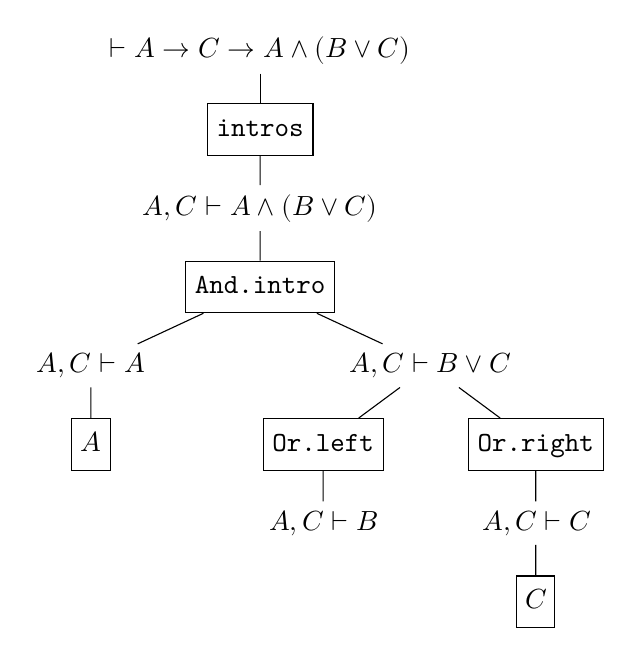
\begin{tikzpicture}[outer sep=auto, level distance=10mm]
      \node {$⊢ A → C → A ∧ (B ∨ C)$}
      child[visible on=<2->] {node[rectangle,draw] {\texttt{intros\strut}}
        child[visible on=<2->] {node {$A, C ⊢ A ∧ (B ∨ C)$}
          child[visible on=<3->] {node[rectangle,draw] {\texttt{And.intro\strut}}
            child[visible on=<3->] {node[xshift=-14mm] {$A, C ⊢ A$}
              child[visible on=<4->] {node[rectangle,draw] {$A\strut$}}}
            child[visible on=<3->] {node[xshift=14mm] {$A, C ⊢ B ∨ C$}
              child[visible on=<5->] {node[rectangle,draw,xshift=-6mm] {\texttt{Or.left\strut}}
                child[visible on=<5->] {node {$A, C ⊢ B$}}}
              child[visible on=<6->] {node[rectangle,draw,xshift=6mm]  {\texttt{Or.right\strut}}
                child[visible on=<6->] {node {$A, C ⊢ C$}
                  child[visible on=<7->] {node[rectangle,draw] {$C\strut$}}}}}}}};
    \end{tikzpicture}
  \end{center}
\end{frame}

\newcommand*{\sprob}[1]{\blue{\textrm{#1\%}}}
\newcommand*{\prio}[1]{{\uncover<2->{\orange{\textrm{#1}\%}}}}

\begin{frame}
  \frametitle{Best-First Tree Search}

  \begin{center}
    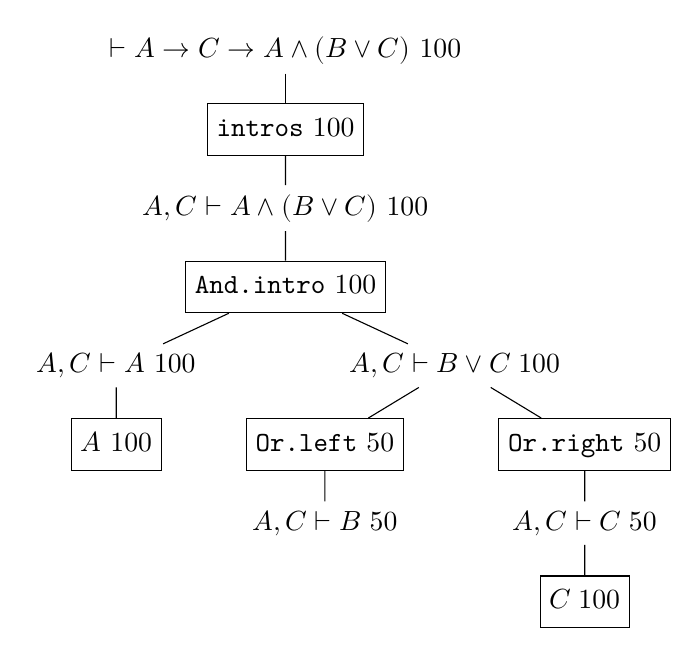
\begin{tikzpicture}[outer sep=auto, level distance=10mm]
      \node {$⊢ A → C → A ∧ (B ∨ C)$ \prio{100}}
      child {node[rectangle,draw] {\texttt{intros\strut} \sprob{100}}
        child {node {$A, C ⊢ A ∧ (B ∨ C)$ \prio{100}}
          child {node[rectangle,draw] {\texttt{And.intro\strut} \sprob{100}}
            child {node[xshift=-14mm] {$A, C ⊢ A$ \prio{100}}
              child {node[rectangle,draw] {$A\strut$ \sprob{100}}}}
            child {node[xshift=14mm] {$A, C ⊢ B ∨ C$ \prio{100}}
              child {node[rectangle,draw,xshift=-9mm] {\texttt{Or.left\strut} \sprob{50}}
                child {node {$A, C ⊢ B$ \prio{50}}}}
              child {node[rectangle,draw,xshift=9mm]  {\texttt{Or.right\strut} \sprob{50}}
                child {node {$A, C ⊢ C$ \prio{50}}
                  child {node[rectangle,draw] {$C\strut$ \sprob{100}}}}}}}}};
    \end{tikzpicture}
  \end{center}
\end{frame}

\begin{frame}
  \frametitle{Safe Rules}

  \begin{itemize}[<+->]
    \item Run before unsafe rules
    \item If a safe rule succeeds on a goal $G$, no other rules are tried for $G$
    \item Treated as 100\% success probability, integer penalty
    \item \good{} Good for performance
    \item \bad{} Users need to make sure that the rule really is safe
  \end{itemize}
\end{frame}

\begin{frame}[fragile]
  \frametitle{Examples}

  \begin{block}{Safe rule: ∧-introduction}
    \begin{rapp}
      \node {$Γ ⊢ \orange{A ∧ B}$}
        child {node {$Γ ⊢ \orange{A}$}}
        child {node {$Γ ⊢ \orange{B}$}};
    \end{rapp}
  \end{block}

  \begin{block}{Unsafe rule: left ∨-introduction}
    \begin{rapp}
      \node {$Γ ⊢ \orange{A ∨ B}$}
        child {node {$Γ ⊢ \orange{A}$}};
    \end{rapp}
  \end{block}
\end{frame}

\begin{frame}
  \frametitle{Normalisation Rules}

  \begin{itemize}[<+->]
    \item Run before safe rules
    \item Treated as 100\% success probability, integer penalty
    \item May produce only one subgoal
    \item Run in a fixpoint loop until no normalisation rule succeeds any more
    \item \good{} Can establish invariants for other rules
    \item \bad{} Typically run multiple times on every goal
    \item Simplifier used as a built-in normalisation rule
  \end{itemize}
\end{frame}

\begin{frame}
  \frametitle{Example}

  \begin{block}{∧-elimination}
    \begin{rapp}
      \node {$Γ,\, \orange{h : A ∧ B} ⊢ T$}
        child {node {$Γ,\, \orange{h₁ : A},\, \orange{h₂ : B} ⊢ T$}};
    \end{rapp}
  \end{block}
\end{frame}

\begin{frame}[fragile]
  \frametitle{Summary: Aesop's Search Algorithm}

  \begin{center}
    \small
    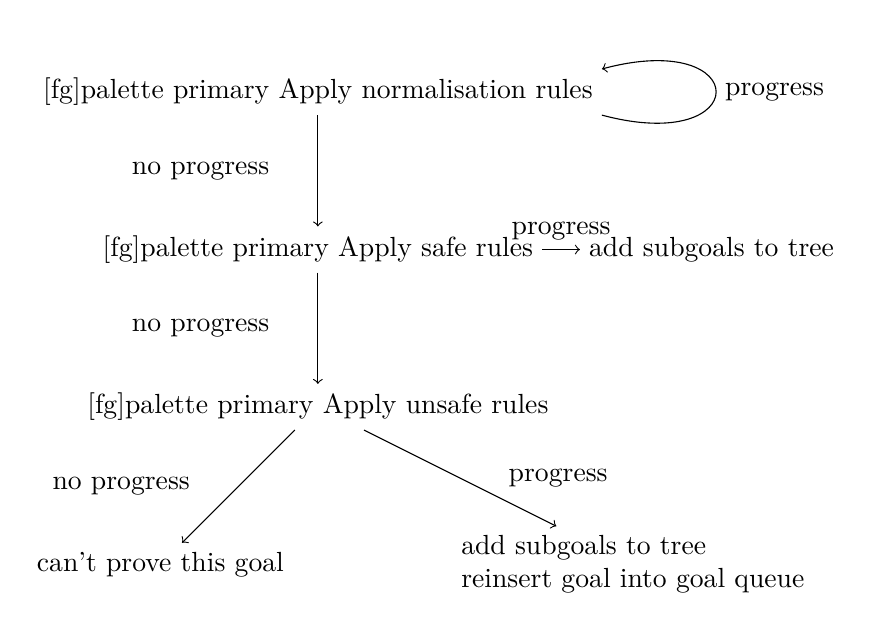
\begin{tikzpicture}[outer sep=auto, norm/.style={}, safe/.style={}, unsf/.style={}]
      \path
        (0,6)  node[norm]            (norm)        {\blue{Apply normalisation rules}}
        (0,4)  node[safe]            (safe)        {\blue{Apply safe rules}}
        (5,4)  node[safe]            (safe-done)   {add subgoals to tree}
        (0,2)  node[unsf]            (unsafe)      {\blue{Apply unsafe rules}}
        (-2,0) node[unsf]            (fail)        {can't prove this goal}
        (4,0)  node[unsf,align=left] (unsafe-done) {add subgoals to tree \\ reinsert goal into goal queue};
      \draw[<-,norm,loop right, min distance=20mm] (norm.{north east}) to node {progress} (norm.{south east});
      \draw[->,safe] (norm) -- node[left,xshift=-5mm] {no progress} (safe);
      \draw[->,safe] (safe) -- node[above] {progress} (safe-done);
      \draw[->,unsf] (safe) -- node[left,xshift=-5mm] {no progress} (unsafe);
      \draw[->,unsf] (unsafe) -- node[left,xshift=-5mm] {no progress} (fail);
      \draw[->,unsf] (unsafe) -- node[right,xshift=5mm] {progress} (unsafe-done);
    \end{tikzpicture}
  \end{center}
\end{frame}

\section{Search with Metavariables}

\begin{frame}[fragile]
  \frametitle{Metavariables}

  \begin{leancode}
    example {a b c d : Nat} (h₁ : a < b)
        (h₂ : a < c) (h₃ : c < d) : a < d := by
      apply Nat.lt_trans
      -- ⊢ a < ?x
      -- ⊢ ?x < d

    example {a b c d : Nat} (h₁ : a < b)
        (h₂ : a < c) (h₃ : c < d) : a < d := by
      aesop (add 1% Nat.lt_trans)
  \end{leancode}
\end{frame}

\begin{frame}
  \frametitle{Challenge: Dependencies Between Goals}

  \begin{tcolorbox}
    \centering
    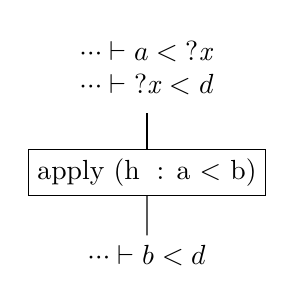
\begin{tikzpicture}[level distance=3em]
      \node {$\begin{array}{l} \dots ⊢ a < \mv{x} \\ \dots ⊢ \mv{x} < d \end{array}$}
        child {node[rectangle,draw,yshift=-0.7em] {\lean{apply (h₁ : a < b)}}
          child {node {$\dots ⊢ b < d$}}};
    \end{tikzpicture}
  \end{tcolorbox}

  \pause

  \begin{tcolorbox}
    \centering
    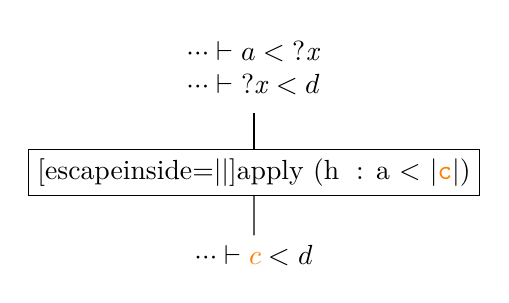
\begin{tikzpicture}[level distance=3em]
      \node {$\begin{array}{l} \dots ⊢ a < \mv{x} \\ \dots ⊢ \mv{x} < d \end{array}$}
        child {node[rectangle,draw,yshift=-0.7em] {{\lean[escapeinside=||]{apply (h₂ : a < |\orange{\texttt{c}}|)}}}
          child {node {$\dots ⊢ \orange{c} < d$}}};
    \end{tikzpicture}
  \end{tcolorbox}
\end{frame}

\begin{frame}
  \frametitle{Challenge: Dependencies Between Goals}

  \begin{tcolorbox}
    \centering
    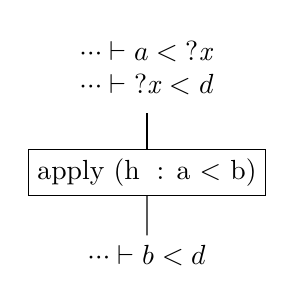
\begin{tikzpicture}[level distance=3em]
      \node {$\begin{array}{l} \dots ⊢ a < \mv{x} \\ \dots ⊢ \mv{x} < d \end{array}$}
        child {node[rectangle,draw,yshift=-0.7em] {\lean{apply (h₁ : a < b)}}
          child {node {$\dots ⊢ b < d$}}};
    \end{tikzpicture}
  \end{tcolorbox}

  \begin{block}{Solution}
    When applying $h₁$ to goal $a < \mv{x}$, consider the resulting second goal $b < d$ a \emph{child} of the rule.
  \end{block}
\end{frame}

\begin{frame}
  \frametitle{Metavariable Paper}

  \fullcite{aesop}
\end{frame}

\section{Proof Script Generation}

\begin{frame}[fragile]
  \frametitle{Proof Script Generation}

  \begin{leancode}
    theorem last_cons {a : α} {l : List α} (h : l ≠ nil) :
        last (a :: l) (cons_ne_nil a l) = last l h := by
      aesop? (add 1% cases List)
  \end{leancode}

  \pause

  \lean{aesop?} generates a proof script:

  \begin{leancode}
    intro h
    cases l with
    | nil =>
      simp_all only [last, ne_eq]
      split
    | cons head tail => simp_all only [last]
  \end{leancode}

  One click replaces \lean{aesop?} with the generated proof.
\end{frame}

\begin{frame}[fragile]
  \frametitle{Challenge: Dynamic Optimisation}

  \begin{block}{Problem}
    For a \lean{simp_all} call, we can \emph{usually, but not always} generate an equivalent \lean{simp_all only [...]} call.
  \end{block}

  \pause

  \begin{block}{Solution}
    Re-execute \lean{simp_all} and \lean{simp_all only [...]}; compare results.
  \end{block}

  \pause

  \begin{block}{Problem}
    Resulting goals are not equal on the nose.
  \end{block}

  \pause

  \begin{block}{Solution}
    A notion of goal equality that abstracts from implementation details.
  \end{block}
\end{frame}

\begin{frame}[fragile]
  \frametitle{Challenge: Reordering}

  \begin{block}{Problem}
    Aesop reports the executed tactics in whatever order it tried them.

    \begin{leancode}
      intro h
      cases l
      on_goal 2 => simp_all only [last]
      simp_all only [last, ne_eq]
      split
    \end{leancode}
  \end{block}

  \pause

  \begin{block}{Solution}
    Reorder tactics to bring them into natural, depth-first order.
  \end{block}
\end{frame}

\begin{frame}
  \frametitle{Challenge: Reordering}

  \begin{block}{Problem}
    When goals contain metavariables, tactic order matters.
  \end{block}

  \pause

  \begin{block}{Solution 1}
    Don't reorder when metavariables are present.
  \end{block}

  \pause

  \begin{block}{Solution 2}
    Try to reorder and check whether the tactics still behave the same.
  \end{block}
\end{frame}

\begin{frame}
  \frametitle{Proof Script Generation Paper}

  \fullcite{script}
\end{frame}

\section{Applications and Shortcomings}

\begin{frame}
  \frametitle{Applications}

  \begin{itemize}[<+->]
    \item General-purpose automation
    \item Domain-specific solvers: \lean{continuity}, \lean{measurability}, \lean{aesop_cat}, \dots
    \item Tree search backend for LLMs\footfullcite{song2023}\footfullcite{abel}
    \item Domain-specific \enquote*{goal preprocessors} with \lean{aesop?}
  \end{itemize}
\end{frame}

\begin{frame}
  \frametitle{Shortcomings}

  \begin{itemize}[<+->]
    \item Built-in logical rules do not deal well with all-quantified hypotheses and sometimes negation
    \item No support for equations beyond \lean{simp}
    \item Default rule set is missing many rules
    \item Repeated calls to \lean{simp} during normalisation are inefficient
  \end{itemize}
\end{frame}

\section{Efficient Forward Reasoning}

\begin{frame}[fragile]
  \frametitle{Forward Rules}

  \begin{leancode}
    @[aesop safe forward]
    theorem pos_of_min_pos_l : 0 < min n m → 0 < n
  \end{leancode}

  \begin{tcolorbox}
    \begin{center}
      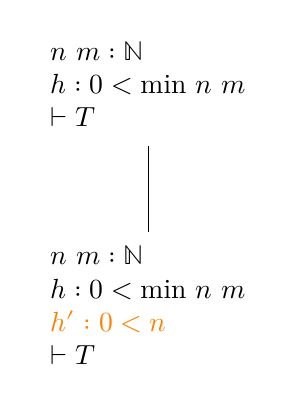
\begin{tikzpicture}[level distance=8em]
      \node {$\begin{array}{l} n~m : ℕ \\ h : 0 < \mathrm{min}~n~m \\ ⊢ T \end{array}$}
        child {node {$\begin{array}{l} n~m : ℕ \\ h : 0 < \mathrm{min}~n~m \\ \orange{h' : 0 < n} \\ ⊢ T \end{array}$}};
      \end{tikzpicture}
    \end{center}
  \end{tcolorbox}
\end{frame}

\begin{frame}[fragile]
  \frametitle{Running Example}

  \begin{leancode}
    axiom R : ℕ → ℕ → Prop

    @[aesop safe forward]
    axiom trans : ∀ x y z, R x y → R y z → R x z

    example
        (h₁ : R 300 301)
        (h₂ : R 301 302)
        (h₃ : R 302 303) :
        R 300 303 := by
      aesop
  \end{leancode}
\end{frame}

\begin{frame}
  \frametitle{Naive Algorithm}

  \begin{enumerate}[<+->]
    \item $R~y~z ≟ R~300~301 ⇒ \{y ↦ 300, z ↦ 301\}$ \good
          \begin{enumerate}[<+->]
            \item $R~x~y ≟ R~300~301 ⇒ \{x ↦ 300, y ↦ 301\}$ \bad
            \item $R~x~y ≟ R~301~302 ⇒ \{x ↦ 301, y ↦ 302\}$ \bad
            \item $R~x~y ≟ R~302~303 ⇒ \{x ↦ 302, y ↦ 303\}$ \bad
          \end{enumerate}
    \item $R~y~z ≟ R~301~302 ⇒ \{y ↦ 301, z ↦ 302\}$ \good
          \begin{enumerate}[<+->]
            \item $R~x~y ≟ R~300~301 ⇒ \{x ↦ 300, y ↦ 301\}$ \good \\
                  \orange{new hypothesis:} $h_{4} : R~300~302$
          \end{enumerate}
  \end{enumerate}
\end{frame}

\begin{frame}[fragile]
  \frametitle{Naive Algorithm}

  \begin{block}{New goal}
    \begin{leancode}
        (h₁ : R 300 301)
        (h₂ : R 301 302)
        (h₃ : R 302 303)
        (h₄ : R 300 302) :
        ⊢ R 300 303
    \end{leancode}
  \end{block}
\end{frame}

\begin{frame}
  \begin{enumerate}[<+->]
    \item $R~y~z ≟ R~300~301 ⇒ \{y ↦ 300, z ↦ 301\}$ \good
          \begin{enumerate}[<+->]
            \item $R~x~y ≟ R~300~301 ⇒ \{x ↦ 300, y ↦ 301\}$ \bad
            \item \dots
          \end{enumerate}
    \item $R~y~z ≟ R~301~302 ⇒ \{y ↦ 301, z ↦ 302\}$ \good
          \begin{enumerate}[<+->]
            \item $R~x~y ≟ R~300~301 ⇒ \{x ↦ 300, y ↦ 301\}$ \orange{already exists}
            \item $R~x~y ≟ R~301~302 ⇒ \{x ↦ 301, y ↦ 302\}$ \bad
            \item \dots
          \end{enumerate}
    \item $R~y~z ≟ R~302~303 ⇒ \{y ↦ 302, z ↦ 303\}$ \good
          \begin{enumerate}
            \item \dots
          \end{enumerate}
  \end{enumerate}
\end{frame}

\begin{frame}
  \frametitle{Central Issue}

  The naive algorithm is \orange{stateless}.

  This leads to lots of \orange{duplicate work}.
\end{frame}

\begin{frame}[fragile]
  \frametitle{Stateful Algorithm Interface}

  \begin{leancode}
    addHyp   : State → Hyp → State × List NewHyp
    eraseHyp : State → Hyp → State
  \end{leancode}
\end{frame}

\begin{frame}
  \frametitle{Rule Anatomy}

  \[
    \mathrm{trans} : ∀ x~y~z~(p₁ : R~x~y)~(p₂ : R~y~z),\, R~x~z
  \]

  $x, y, z$ are determined by a match for $p₁$ and $p₂$.

  $p₁$ and $p₂$ are the \emph{slots} of $\mathrm{trans}$.

  They are connected by the \emph{shared variable} $y$.
\end{frame}

\begin{frame}
  \frametitle{Matches}

  \[
    \mathrm{trans} : ∀ x~y~z~(p₁ : R~x~y)~(p₂ : R~y~z),\, R~x~z
  \]

  A \emph{complete match} for $\mathrm{trans}$ is a substitution
  \[
    \{1 ↦ t, 2 ↦ u\}
  \]
  such that $t : R~a~b$ (matching $p₁$) and $u : R~c~d$ (matching $p₂$) with $b = c$.

  A \emph{partial match} is a substitution for some nonempty subset of the slots.
\end{frame}

\begin{frame}
  \frametitle{Core Algorithm Idea}

  \emph{Iteratively fill the matches}: find a hypothesis for slot 1, then find a hypothesis for slot 2 that agrees on the shared variables, \dots

  When a new hypothesis comes in, \emph{extend the matches} that agree with this hypothesis.

  \emph{Store the partially filled matches} in the state.
\end{frame}

\begin{frame}
  \frametitle{Rule State}

  The \emph{rule state} for $\mathrm{trans}$ is a pair of maps
  \begin{align*}
    H &: \Slots × \Vars × \Expr → \Pow{\Hyps} \\
    M &: \Slots × \Vars × \Expr → \Pow{\Matches}
  \end{align*}
  where
  \begin{itemize}
    \item \Slots{} is the set of slot indices of $\mathrm{trans}$ (here $\Slots = \{1,2\}$)
    \item \Vars{} is the set of variables shared between the slots (here $\Vars = \{y\}$)
    \item \Expr{} is the set of Lean terms
    \item \Hyps{} is the set of hypotheses
    \item \Matches{} is the set of partial matches for $\mathrm{trans}$
  \end{itemize}
\end{frame}

\begin{frame}
  \frametitle{Hypothesis Map}

  For a hypothesis $h$, slot $s$, variable $v$, expression $e$:

  $h ∈ H(s, v, e)$ iff \\
  the type of $h$ matches the type of slot $s$ \\
  with variable $v$ instantiated by $e$.

  \begin{example}
    Given $h₁ : R~300~301$
    \begin{align*}
      h₁ &∈ H(1, y, 301) \\
      h₁ &∈ H(2, y, 300) \\
    \end{align*}
  \end{example}
\end{frame}

\begin{frame}
  \frametitle{Match Map}

  For a hypothesis $h$, slot $s$, variable $v$, expression $e$:

  $m ∈ M(s, v, e)$ iff \\
  all slots $≤ s$ are assigned in $m$ \\
  all slots $> s$ are unassigned in $m$ \\
  with variable $v$ instantiated by $e$.

  \begin{example}
    Given $h₁ : R~300~301$, $m = \{1 ↦ h₁\}$
    \begin{align*}
      m &∈ M(1, y, 301) \\
    \end{align*}
  \end{example}
\end{frame}

\begin{frame}
  \frametitle{Adding a Hypothesis: Example}

  $\mathrm{trans} : R~x~y → R~y~z → R~x~z$ \\
  $h₂ : R~301~302$, $h₁ : R~300~301$, $h₃ : R~302~303$

  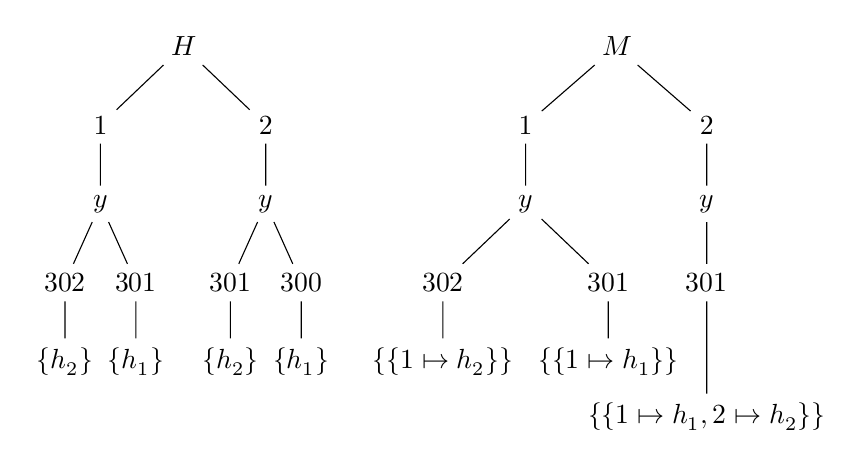
\begin{tikzpicture}[outer sep=auto, level distance=10mm]
    \node {$H$}
      child {node[xshift=-.3cm] {1}
        child[] {node {$y$}
          child[visible on=<2->] {node[xshift=.3cm] {$302$}
            child {node {$\{h₂\}$}}}
          child[visible on=<5->] {node[xshift=-.3cm] {$301$}
            child {node {$\{h₁\}$}}}}}
      child {node[xshift=.3cm] {2}
        child {node {$y$}
          child[visible on=<4->] {node[xshift=.3cm] {$301$}
            child {node {$\{h₂\}$}}}
          child[visible on=<8->] {node[xshift=-.3cm] {$300$}
            child {node {$\{h₁\}$}}}}};
    \node[xshift=5.5cm] {$M$}
      child {node[xshift=-.4cm] {1}
        child {node {$y$}
          child[visible on=<3->, xshift=-.3cm] {node {$302$}
            child {node {$\{\{1 ↦ h₂\}\}$}}}
          child[visible on=<6->, xshift=.3cm] {node {$301$}
            child {node {$\{\{1 ↦ h₁\}\}$}}}}}
      child {node[xshift=.4cm] {2}
        child {node {$y$}
          child[visible on=<7->] {node {$301$}
            child {node[yshift=-2em] {$\{\{1 ↦ h₁, 2 ↦ h₂\}\}$}}}}};
  \end{tikzpicture}
\end{frame}

\begin{frame}
  \frametitle{Adding a Hypothesis: Algorithm}

  Given a new hypothesis $h : T$, \\
  for each slot $s$ such that $T$ matches the type of $s$:
  \begin{enumerate}
    \item Add $h$ to $H(s, v, e)$ for each shared variable $v$.
    \item Get the matches in slot $s-1$ that agree with $h$ on the shared
          variables.
          Extend these matches with $h$ and add them to $M(s, v, e)$ for each $v$.
    \item For each extended match $m$, get the hypotheses in slot $s + 1$ that
          agree with $m$. Extend the matches again and add them to $M$.
    \item Repeat with slots $s + 2$, $s + 3$, \dots
    \item If a match is completed, report it as a new hypothesis.
  \end{enumerate}
\end{frame}

\begin{frame}
  \frametitle{Benchmark}

  % TODO
\end{frame}

\begin{frame}
  \centering{\Huge{\blue{Thanks!}}}
  % TODO Links/QR codes for these slides, Aesop repo, my CV
\end{frame}

\end{document}
